\documentclass[letter,11pt]{article}

\usepackage{titlesec}
\usepackage{graphicx}
\usepackage{caption}
\usepackage{subcaption}
\usepackage{amsmath}
\usepackage{amsfonts}
\usepackage{amssymb}
\usepackage{hyperref}
\usepackage{enumitem}
\usepackage{listings}
\usepackage{xcolor}

% Define colors for syntax highlighting
\definecolor{mygreen}{rgb}{0,0.6,0}
\definecolor{mygray}{rgb}{0.5,0.5,0.5}
\definecolor{mymauve}{rgb}{0.58,0,0.82}

% Set up the MATLAB code listing style
\lstset{
  backgroundcolor=\color{white},
  basicstyle=\footnotesize\ttfamily,
  breakatwhitespace=false,
  breaklines=true,
  captionpos=b,
  commentstyle=\color{mygreen},
  deletekeywords={...},
  escapeinside={\%*}{*)},
  extendedchars=true,
  frame=single,
  keepspaces=true,
  keywordstyle=\color{blue},
  language=Matlab,
  otherkeywords={*,...},
  numbers=left,
  numbersep=5pt,
  numberstyle=\tiny\color{mygray},
  rulecolor=\color{black},
  showspaces=false,
  showstringspaces=false,
  showtabs=false,
  stepnumber=1,
  stringstyle=\color{mymauve},
  tabsize=2,
  title=\lstname
}


% Adjust the margins if needed
\usepackage[left=1in, right=1in, top=1in, bottom=1in]{geometry}
\usepackage{graphicx}
\usepackage{graphicx}
\usepackage{tabto}

% Set the title and author
\title{Iteration and Error}
\author{David Tran and Spencer Kelly}
\date{\today}

\begin{document}

\maketitle

\subsection*{Abstract}

\subsection*{Introduction}
In the field of numerical analysis, one of the first important concepts introduced is the idea of approximating otherwise complex and computationally expensive to evaluate functions using much simpler and efficient methods.
In this lab, the first of four, we delve into the approximations of functions using their Taylor series and their associated Taylor remainders, exposing the reader to introductory concepts in functional approximation.

Taylor series are a powerful tool in mathematics, and provide us with a means of representing a smooth function using an infinite series of polynomial terms.
These series allow us to work with otherwise difficult functions, and have applications in a variety of fields including physics, engineering, and quantitative finance, where they aid in modeling complex systems, solving differential equations, and the analysis of complex functions, to name a few.

For the purposes of computation, it is not realistic to use the infinite taylor series for a given function.
In this lab, we introduce the truncated (finite terms) Taylor series for a single function.
We will compare the truncated Taylor series to the function in which it approximates, and analyze the difference between the two, over various domains.
We will also analyze the Taylor remainder, which represents the error associated with truncation to finite terms.
By analyzing the differing number of terms before truncation and plotting the Taylor remainder, we can observe how the degree of truncation effects the accuracy of the approximation, providing insight into the tradeoff between efficiency and accuracy in the field of numerical analysis.

The field of numerical analysis in some form dates back over 2000 years ago in ancient Egypt, and there is evidence to suggest that Babylonians may have used numerical methods to calculate the square root of 2 to within 5 decimal places.
Though using more modern methods, and with the help of the computational software MATLAB, this lab serves as an introduction to methods of computation and approximation in numerical analysis that have been of great use across many fields and civilizations.

\subsection*{Particular aspects of this Lab }

\subsection*{Taylor series and error}
\subsubsection*{Problem 0}
Let $f(x) = e^{-x}$. Note that $f^{(1)}(x) = -e^{-x}, f^{(2)}(x) = e^{-x}$, and in general, $f^{(n)}(x) = (-1)^ne^{-x}$. So, $f^{(n)}(0) = (-1)^n$, and the Taylor series expansion around $x_0 = 0$ is given by

\begin{align*}
T_n(x) &= \sum_{k = 0}^n \frac{f^{(k)}(x_0)}{k!} x^k \\
&= \sum_{k = 0}^n \frac{(-1)^k}{k!}x^k
\end{align*}

THIS IS SPENCER;

Similarily, the remainder term is

\begin{align*}
R_n &= \frac{f^{(n + 1)}(z)}{(n + 1)!}(x - x_0)^{n + 1} \\
&= \frac{(-1)^{n + 1} e^{-c}}{(n + 1)!}x^{n + 1}.
\end{align*}

for some $0 \leq c \leq x$.

\subsubsection*{Problem 1}
\begin{enumerate}[label=\alph*.]
  \item We have \begin{align*}
    e^{-x} &= 1 - x + \frac{x^2}{2!} - \frac{x^3}{3!} + \dots
  \end{align*}
  so
  \begin{align*}
    F(x) &= \frac{e^{-x} - 1 + x}{x^2} \\
    &= \frac{1}{2!} - \frac{x}{3!} + \frac{x^2}{4!} - \dots \\
    &= \sum_{k = 0}^\infty (-1)^k \frac{x^k}{(k + 2)!}
  \end{align*}

  and its Taylor series up to $n + 1$ terms is

  $$
  T_n(x) = \sum_{k = 0}^n (-1)^k \frac{x^k}{(k + 2)}
  $$

  To find the remainder term $R_n$, we use the fact that $R_n = F(x) - T_n(x)$. TODO.
  \item TODO.
\end{enumerate}

\subsubsection*{Problem 2}
\begin{enumerate}[label=\alph*.]
  \item We compute and plot $F(x)$ from above with the following.

  \lstinputlisting{F.m}

  \item TODO.
\end{enumerate}

\subsubsection*{Problem 3}
\begin{enumerate}[label=\alph*.]
  \item TODO.
  \item TODO.
  \item TODO.
  \item TODO.
\end{enumerate}

\subsubsection*{Problem 4}
\begin{enumerate}[label=\alph*.]
  d. Below is the plot of the domain from problem 2 done using the function myfofxv2.m, which uses a taylor series expansion
to plot x values between -10^{-7} and 10^{-7}. If the value falls not between those bounds, then the functions opts for the original form of the function.

\begin{figure}[htbp]
\centering
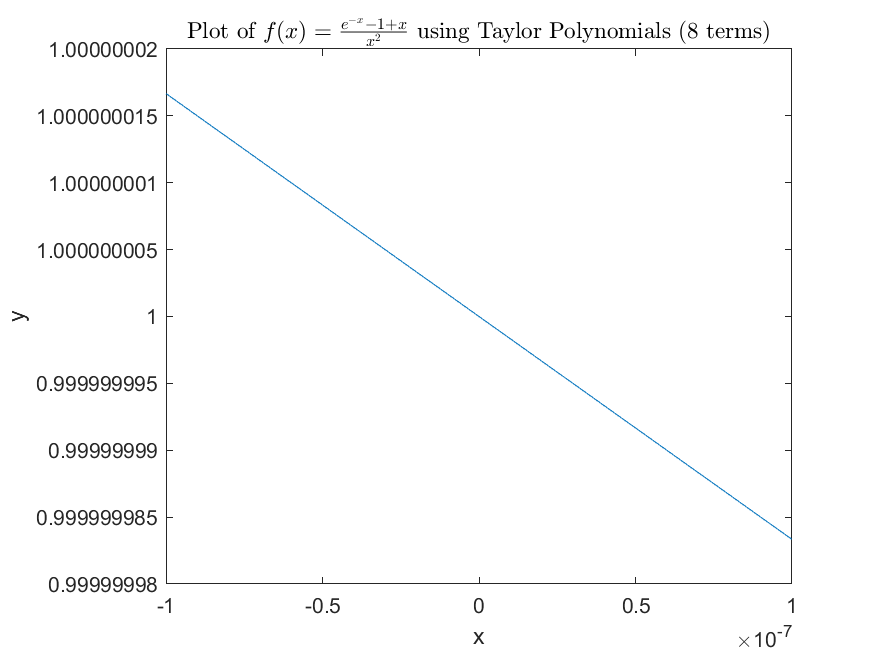
\includegraphics[width=\linewidth]{Lab1BQ4p1q2}  % Adjust the file name and extension
\caption{Caption of your figure.}
\label{Plot of the domain from problem 2 using the function}
\end{figure}
  \\

  Below is the plot of the domain from problem 3, using the same function:

  \begin{figure}[htbp]
\centering
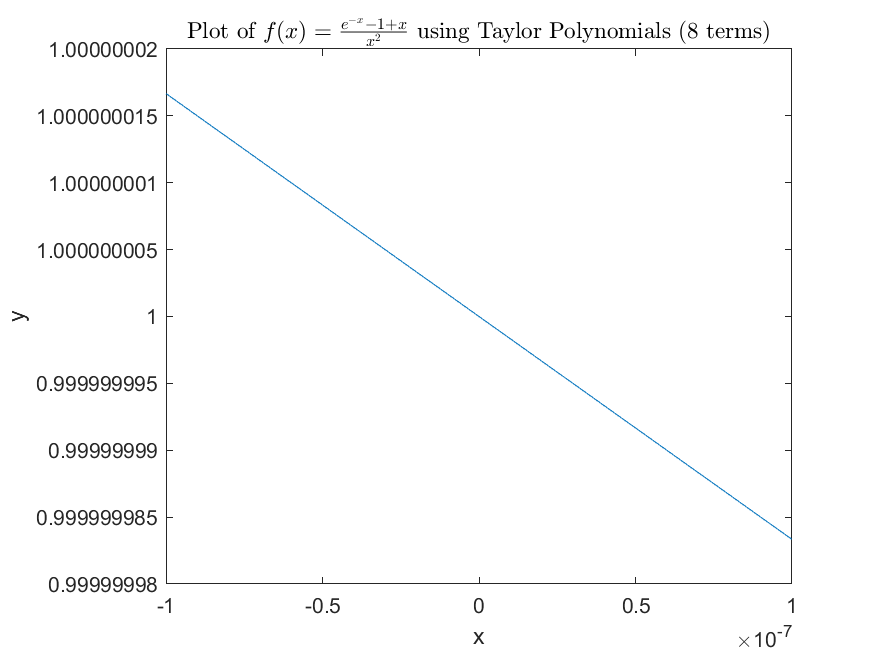
\includegraphics[width=\linewidth]{Lab1BQ4p1q3}  % Adjust the file name and extension
\caption{Caption of your figure.}
\label{Plot of domain from problem 3 using the same function}
\end{figure}

\end{enumerate}

\subsection*{Summary and Conclusions}

\begin{thebibliography}{99}
  % Add your references here using the \bibitem{} command
  % Example: \bibitem{author_year} Author, A., \& Year, Y. Title of the paper. \textit{Journal Name}, \textbf{Volume}(Issue), PageRange.
\end{thebibliography}

\subsection*{Teamwork Statement}

\subsection*{Code Appendix}

\subsection*{Plot Appendix}


\subsection*{References}\\

  \tab Garcia, A. L. (2015). Numerical Methods for Physics. CreateSpace.\\

  Leblanc, F. (2010). An introduction to Stellar Astrophysics. John Wily & Sons.\\

  King, G. C. (2010). Vibrations and Waves. John Wiley & Sons.



\end{document}
